% Intended LaTeX compiler: pdflatex
\documentclass[11pt,a4paper,final]{article}
\usepackage[a4paper, total={7in, 10in}]{geometry}
\usepackage{algorithm2e}
\usepackage{booktabs}
\usepackage{fancyhdr}
\usepackage{graphicx}
\usepackage{hyperref}
\usepackage{subcaption}
\usepackage{tikz}
\usepackage[utf8]{inputenc}
\usepackage[T1]{fontenc}
\usepackage{graphicx}
\usepackage{longtable}
\usepackage{wrapfig}
\usepackage{rotating}
\usepackage[normalem]{ulem}
\usepackage{amsmath}
\usepackage{amssymb}
\usepackage{capt-of}
\usepackage{hyperref}
\pagestyle{fancy}
\fancyhead{}
\rhead{\textit{Alexander Brown}}
\lhead{\textit{ECE 6030}}
\small
\usepackage{amsfonts}                       % Cool math fonts
\usepackage{amsmath}                        % Maths
\setlength\parindent{0pt}                   % No indent for paragraphs
\newcommand{\shall}{\textbf{shall }}
\author{Alexander Brown}
\date{\today}
\title{Homework 1}
\hypersetup{
 pdfauthor={Alexander Brown},
 pdftitle={Homework 1},
 pdfkeywords={},
 pdfsubject={},
 pdfcreator={Emacs 28.2 (Org mode 9.5.5)}, 
 pdflang={English}}
\begin{document}

\maketitle
\setcounter{secnumdepth}{-1}

\parskip 3mm                                % Set the vetical space between paragraphs
\let\ref\autoref                            % Redifine `\ref` as `\autoref` because lazy

\section{1}
\label{sec:org0c71b5b}
Thoughtfully read

\section{2}
\label{sec:org09c0061}

\subsection{Nonlinear Feedback Design for Fixed-Time Stabilization of Linear Control Systems}
\label{sec:org89c7237}
The title of the paper is quite colorful in the description of the paper as it paints the full picture. It introduces
finite time controllers for global-finite time stability of closed loop systems and a guaranteed convergence time of
system trajectories into a neighborhood. These controllers are of two different "types". Having taken nonlinear control
and optimal control that math does not look foreign, but there is a whole lot in this paper. With time I could probably
get through it.

\subsection{Cooperative Output Feedback Tracking Control of Stochastic Linear Heterogeneous Multiagent Systems}
\label{sec:org3fc276e}
This paper is an odd one. It has a set of heterogeneous leaders and followers. Each agent has incomplete
measurable dynamics, so they propose a set of observation strategies to be able to predict the states of the collective.
Again, this is a long paper with a lot of dynamics. I have taken a multiagent systems course, optimal estimation, and
the previously mentioned courses in control. With time, I could probably get though the paper.

\subsection{Time-Variation in Online Nonconvex Optimization Enables Escaping From Spurious Local Minima}
\label{sec:orgc7b1f5f}
This paper alludes me. I understand what meant when they throw out nonconvex optimization, stability analysis, and
time-varying optimization, but that is about as far as I go. I believe the goal is to use something similar to that of a
gradient search for time dependent systems. They are allowing the gradient to vary with time and include inertial terms
as to not allow the line the algorithm is tracking to be immediately swayed by any change to the system.

\section{3}
\label{sec:org7158cf0}
\subsection{Problem Statement}
\label{sec:org1844730}
Show that the following are convex:

\begin{enumerate}
\item The set of \(n \times n\) Toeplitz matrices
\item The set of monic polynomials of the same degree
\item The set of symmetric matrices
\end{enumerate}

\subsection{Solution}
\label{sec:org719eedd}
Begin by defining what a complex set is:

\begin{quote}
A set \(S\) is convex if for any two points \(p,q \in S\), then all points of the form

$$
\lambda p + (1 - \lambda)q
$$

for \(0 \le \lambda \le 1\), are also in \(S\).
\end{quote}

\subsubsection{3.1: Toeplitz}
\label{sec:3.1}
Begin by defining what a Toeplitz matrix is

\begin{quote}
A Toeplitz matrix is a diagonal-constant matrix, which means all elements along a diagonal have the same value. For a
Toeplitz matrix \(A\) we have \(A_{ij} = a_{i-j}\) which results in the form

\begin{equation*}
\begin{bmatrix}
a & b & c & \cdots \\
e & a & b & \cdots \\
f & e & a & \cdots \\
\vdots & \vdots & \vdots & \ddots
\end{bmatrix}
\end{equation*}
\end{quote}

Consider Toeplitz matrices \(P\) and \(Q\) of dimension \(n \times n\) as let \(S\) be the set of \(n\times n\) Toeplitz matrices. Lets now apply the definition of the convex set:

$$
\lambda P + (1 - \lambda)Q
$$

There are two operations being applied to the matrices: addition

\begin{quote}
If \(A = [a_{ij}]\) and \(B = [b_{ij}]\) are matrices of the same size, then their sum \(A+B\) is the matrix obtained by
adding the corresponding elements of the matrix \(A\) and \(B\).
\end{quote}

and multiplication of a matrix by a number

\begin{quote}
If \(A = [a_ij]\) is a matrix and \(c\) is a number, then \(cA\) is the matrix obtained by multiplying each element of \(A\) by
\(c\).
\end{quote}

Therefore, we can make the statements

\begin{itemize}
\item Any Toeplitz matrix multiplied by a scalar is also Toeplitz
\item Any two \(n \times n\) Toeplitz matrices being added together is also Toeplitz
\end{itemize}

The following statement can then be made: The set of \(n \times n\) Toeplitz matrices is convex.

$$
\lambda P + (1 - \lambda)Q \in S
$$

\subsubsection{3.2: Monic Polynomials of Degree \(n\)}
\label{sec:org251cd56}
Begin by defining what a monic polynomial is

\begin{quote}
A polynomial is monic if the coefficient of the highest order term is 1.
\end{quote}

Suppose \(p\) and \(q\) are monic polynomials of degree \(n\) and \(S\) is the set of all monic polynomials of degree \(n\). It
can be written

$$
\lambda p(x) + (1 - \lambda)q(x) \in S
$$

Expanding the above gives

\begin{equation*}
\begin{array}{l}
\lambda (x^n - ax^{n-1} + \cdots + bx + c) + (1- \lambda)(x^n + dx^{n-1} + \cdots + ex + f) \\
= 2 \lambda x^n + (a+d x^{n-1}) + \cdots \\
\end{array}
\end{equation*}

Dividing by \(2\lambda\) produces another monic polynomial of degree \(n\). Therefore, the set is convex, i.e \(\lambda p(x) + (1 - \lambda)q(x) \in S\).

\subsubsection{3.3: Symmetric Matrices}
\label{sec:orgc0214b7}
Define what a symmetric matrix is

\begin{quote}
A matrix \(A\) is symmetric \(\iff A = A^T\).
\end{quote}

Similarly to \hyperref[sec:3.1]{3.1},

\begin{itemize}
\item Let \(P\) and \(Q\) are \(n \times n\) symmetric matrices
\item \(S\) is the set of \(n \times n\) symmetric matrices
\item Any symmetric matrix multiplied by a scalar is also symmetric
\item Any two \(n \times n\) symmetric matrices being added together is also symmetric
\end{itemize}

Therefore, \(S\) is convex because \(\lambda P + (1 - \lambda)Q \in S\).

\section{4}
\label{sec:org87f357f}
\subsection{Problem Statement}
\label{sec:org7daabd1}
The set of even integers can be represented as \(2\mathbb{Z}\). Show that \(|2\mathbb{Z}| = |\mathbb{Z}|\). Similarly show that there are as many odd
integers as there are integers.

\subsection{Solution}
\label{sec:org4a1c6a8}
Let \(S\) and \(T\) be two different sets. \(T\) and \(S\) have the same cardinality if there is a bijection \(f\) from \(S\) to
\(T\). Therefore, we need to show \(f : \mathbb{Z} \rightarrow 2\mathbb{Z}\). Let the mapping \(f(n)\) be defined as

\begin{equation*}
f(n) = 2n
\end{equation*}

It now needs to be shown that \(f(n)\) is both one-to-one and onto. To show that \(f(n)\) is one-to-one begin by defining
how to show a mapping is one-to-one

\begin{quote}
A function \(f\) from \(A\) onto \(B\) is one-to-one if each element of \(B\) has at most one element of \(A\) mapped into it.
That is, \(f(x) = f(y)\), then \(x = y\).
\end{quote}

From this if we suppose \(f(a) = f(b)\), then \(2a = 2b\) so \(a=b\). Thus, \(f\) is one-to-one. Now we need to show \(f\) is
onto. Begin by defining onto

\begin{quote}
A function is onto if each element of \(B\) has at least one element of \(A\) that is mapped into it. That is, \(\forall b
\in B\) there is an \(a \in A\) such that \(f(a) = b\).
\end{quote}

Take \(b = 2n\) for some \(a\), then \(f(n) = 2n = b\) which shows that \(f\) is onto. Therefore, \(f(n)\) is a bijection and
\(|\mathbb{Z}| = |2\mathbb{Z}|\).

Similarly, for the odd we need to show \(f : \mathbb{Z} \rightarrow 2\mathbb{Z}+1\) is a bijection. To show \(f(n)\) is one-to-one let \(f(a) = f(b)\),
then \(2a + 1 = 2b + 1\), so \(a=b\). To show \(f\) is onto let \(b = 2n+1\), then \(f(n) = 2n + 1 = b\). Therefore, \(f(n)\) is a
bijection and \(|\mathbb{Z}| = |2\mathbb{Z}+1|\).

\section{5}
\label{sec:org2b58a6e}

\subsection{Problem Statement}
\label{sec:org8b364b7}
Show that \(|(0,1]| = |\mathbb{R}|\).

\subsection{Solution}
\label{sec:org6115038}
A simple way to go about this is to first show that \(\big|[0,1)\big| = \big|[-\pi/2, \pi/2)\big|\). Suppose \(f(x) = \pi x - \pi/2\). To show that
\(f(x)\) is one-to-one

\begin{equation*}
\begin{array}{l}
f(x) = f(y) \\
\pi x - \pi/2 = \pi y - \pi/2 \\
\pi x = \pi y \\
x = y
\end{array}
\end{equation*}

Therefore, \(f(x)\) is one-to-one. Now to show that \(f(x)\) is also onto.

\begin{equation*}
\begin{array}{l}
f(x) = y \\
\pi x - \pi / 2 = y \\
x = y/\pi + 1/2
\end{array}
\end{equation*}

And because we know that \(0 < x \le 1\) we can show that \(x\) written above is in that range by saying

\begin{equation*}
\begin{array}{l}
- \pi/2 < y \le \pi/2 \\
- 1/2 < y/\pi \le 1/2 \\
0 < y/\pi + 1/2 \le 1\\
\end{array}
\end{equation*}

Therefore, the function is also onto. Now to show that \(\big|[-\pi/2, \pi/2)\big| = \big| \mathbb{R} \big|\). Let \(g(x) = tan(x)\) it
can be shown that \(tan(x)\) is always increasing.

\begin{quote}
\textbf{Fact}: If \(g(x)\) is always increasing, then \(g(x)\) is one-to-one.
\end{quote}

By taking the derivative of \(g'(x) = sec^2(x) > 0\), therefore \(g(x)\) is one-to-one. To show that \(g(x)\) is onto, we will
use the intermediate value theorem

\begin{quote}
If \(g(x)\) is continuous on an interval \([a,b]\), then \(g(x)\) contains all the values between \(g(a)\) and \(g(b)\).
\end{quote}

Let the range of interest be \([-\pi/2 + \epsilon, \pi/2 - \epsilon]\). \(g(x)\) is continuous within the range, therefore it obtains all
values \(g(-\pi/2 + \epsilon)\) to \(g(\pi/2 - \epsilon)\). If we let \(\epsilon \rightarrow 0\) then \(g(x) \rightarrow \mathbb{R}\). Therefore, \(\big|(0,1]\big| = \big| \mathbb{R} \big|\).

\section{6}
\label{sec:org60e5cfd}
\subsection{Problem Statement}
\label{sec:orge087fd5}
Show that the intersection of a convex set is convex.

\subsection{Solution}
\label{sec:org01dbe53}
Let \(A\) and \(B\) be two convex sets, and let \(C = A \cup B\). Now let \(p,q \in C\).

\begin{itemize}
\item If \(p,q \in C\) then \(p,q \in A\) and \(A\) is convex
\item If \(p,q \in C\) then \(p,q \in B\) and \(B\) is convex
\item Therefore \(C\) must be complex
\end{itemize}

\section{7}
\label{sec:org5f6827c}
\subsection{Problem Statement}
\label{sec:org67a899e}
If \(S\) and \(T\) are convex sets both in \(\mathbb{R}^n\), show that the set sum is convex.

\begin{center}
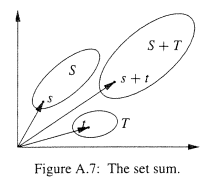
\includegraphics[width=0.45\textwidth]{./img/set-sum.png}
\end{center}

\subsection{Solution}
\label{sec:orgeb367c2}
The set sum is defined as

$$
S+T = \{x: x = s + t, s\in S, t \in T\}
$$

Let \(S\) and \(T\) be convex sets and \(S+T \in C\), let \(s_1, s_2 \in S\) and \(t_1, t_2 \in T\), and let \(s = s_1 + t_1\) and \(t = s_2 + t_2\), then

\begin{equation*}
\lambda s + (1 - \lambda)t \\
\lambda s_1 + \lambda t_1 + s_2(1-\lambda) + t_2(1-\lambda) \\
\lambda s_1 + (1-\lambda)t_1 + \lambda s_2 + (1-\lambda) t_2 \in C \\
\end{equation*}

Therefore, the set sum is convex.

\section{8}
\label{sec:1.8}
\subsection{Problem Statement}
\label{sec:org61070b3}
Show that the polytope in \(n\) dimensions is defined by

\begin{equation*}
P_n = \{ x \in \mathbb{R}^n : x_i \ge 0, \sum_{i=1}^n x_i = 1 \}
\end{equation*}

\subsection{Solution}
\label{sec:org38da342}
Let is take the case of \(n=1\) to start. Let \(p = x1\) and \(q = y_1\) then
using the definition used before we get

$$
\lambda p + (1 - \lambda)q
$$

Which must be convex because it is a single point. Now let \(n=3\)

\begin{equation*}
\begin{array}{c}
\lambda p + (1 - \lambda)q \\
\lambda (x_1, x_2, x_3) + (1 - \lambda)(y_1, y_2, y_2) = (z_1, z_2, z_3)\\
\end{array}
\end{equation*}

Because \(z\) must add up to 1, the set must be convex.

\section{9}
\label{sec:orgfc784fd}
\subsection{Problem Statement}
\label{sec:org8a6e796}
For the polytope \(P_n\) of the previous problem, let \((a_1, a_2, \cdots, a_n) \in P_n\). Show by induction that

$$
n^2 \le \sum_{i=1}^n \frac{1}{a_i}
$$

\subsection{Solution}
\label{sec:org823dc79}
Begin with the base case, \(n=1\).

\begin{equation*}
\begin{array}{c}
1^2 \le \sum_{i=1}^1 \frac{1}{1} \\
1 \le 1
\end{array}
\end{equation*}

which is true. Now let

$$
n^2 \le \sum_{i=1}^n \frac{1}{a_i}
$$

be true. We now need to show that the following is true

$$
(n+1)^2 \le \sum_{i=1}^{n+1} \frac{1}{a_i}
$$

Begin by defining an element from \(P_N\): \(p = (a_1, a_2, \cdots, a_n)\). To make \(p\) an element in the \(P_{n+1}\) space let \(p
= (a_1, a_2, \cdots, a_n, 0)\). Let's define another point \(q = (0, 0, \cdots, 0, 1)\). Now let's define the line between the points
\(p\) and \(q\)

\begin{equation*}
\begin{array}{c}
\lambda p + (1 - \lambda)q \\
\lambda (a_1, a_2, \cdots, a_n, 0) + (1 - \lambda)(0, 0, \cdots, 0, 1) = (b_1, b_2, \cdots, b_{n+1}) \\
\end{array}
\end{equation*}

Going back to the \((n+1)^2 \le \sum_{i=1}^{n+1} \frac{1}{a_i}\), let's plug this in for \(b\) for \(a\): \((n+1)^2 = \sum_{i=1}^{n+1}
\frac{1}{b_i}\). Note that the \((1-\lambda)\) is non-zero at \(n+1\), so we can rewrite this as \((n+1)^2 = \frac{1}{1-\lambda} + \sum_{i=1}^{n+1}
\frac{1}{\lambda a_i}\). Now to remove the \(\lambda\):

\begin{equation*}
\frac{1}{1-\lambda} + \sum_{i=1}^{n+1} \frac{1}{\lambda a_i} \le \sum_{i=1}^{n+1} \frac{1}{a_i} \\
\end{equation*}

Therefore, \((n+1)^2 \le \sum_{i=1}^{n+1} \frac{1}{a_i}\).

\section{10}
\label{sec:orgefd82ba}
\subsection{Problem Statement}
\label{sec:org26caa07}
Show that \((AB)^T = B^T A^T\) is true.

\subsection{Solution}
\label{sec:orgb82f68d}
Let \(A\) be a \(m \times n\) matrix and \(B\) be a \(n \times p\) matrix. And let \(A = (a_{ij})\) and \(A^T = (a_{ji})\), the same can be
said for \(B\). If we look at the multiplication of \((AB)^T\)

$$
(AB)^T = \sum_{k=1}^n (a_{ik} b_{ki})^T
$$

Which denotes the row/column multiplication/addition of matrix multiplication for transposed matrices. Now if we
transpose the summed values

$$
(AB)^T = \sum_{k=1}^n (a_{ik} b_{ki})^T = \sum_{k=1}^n (a_{kj} b_{ki})
$$

Reversing the multiplication order we get

$$
(AB)^T = \sum_{k=1}^n (b_{ki} a_{kj})^T = B^T A^T
$$

\section{11}
\label{sec:orgff45df0}
\subsection{Problem Statement}
\label{sec:org6d6e416}
Show that the following are true

\subsection{Solution}
\label{sec:org7ab93fc}

\subsubsection{\(A_{i:} = \sum_j a_{ij}e_{j}\)}
\label{sec:orgeed3aa4}
Begin with definition of unit vectors

\begin{equation*}
\begin{array}{ccc}
e_1 =
\begin{bmatrix}
1 \\ 0 \\ 0 \\ \vdots \\ 0
\end{bmatrix}
e_2 =
\begin{bmatrix}
0 \\ 1 \\ 0 \\ \vdots \\ 0
\end{bmatrix}
e_n =
\begin{bmatrix}
0 \\ 0 \\ 0 \\ \vdots \\ n
\end{bmatrix}
\end{array}
\end{equation*}

Now outline the form of \(A_{i:} = [a_{i1},a_{i2},a_{i3},\cdots,a_{in}]\) which denotes the all the elements of row \(i\). To
show that is equivalent to the sum, begin by expanding the sum. Let \(k\) be the column of interest.

\begin{equation*}
\sum_j a_{ij}e_j = a_{i1}e_1 + a_{i2}e_2 + \cdots + a_{ik}e_{k} + a_{in}e_n
\end{equation*}

Referring back to the definition of \(e\), we see that only \(e_k\) is nonzero therefore the only value returned is
\(a_{ik}\). Extrapolating this for all columns \(n\) in the matrix we get the vector \([a_{i1},a_{i2},a_{i3},\cdots,a_{in}]\).

\subsubsection{\(A_{:j} = \sum_i a_{ij}e_{i}\)}
\label{sec:org2ec84aa}
This is very similarly to the previous problem; however, now we are summing over the columns. \(A_{:j} = [a_{1j},a_{2j}
\cdots,a_{mj}]^T\). Now taking the sum version, we find

\begin{equation*}
\sum_i a_{ij}e_i = a_{1j}e_1 + a_{2j}e_2 + \cdots + a_{kj}e_{k} + a_{nj}e_m
\end{equation*}

Where the only nonzero value in \(e\) is \(e_k\), therefore we are returned \(a{kj}\) when \(i=k\). Doing this for all \(m\)
elements returns the vector \([a_{1j},a_{2j},\cdots,a_{mj}]^T\)

\subsubsection{\(A_{i:}^T = \sum_j a_{ij}e_{j}^T\)}
\label{sec:org8f23db5}
This is nearly the same as \(A_{i:} = \sum_j a_{ij}e_{j}\), but now because \(A\) is transposed, the unit vectors must also be
transposed to keep the dimensions connect (column vector to row). Therefore, in a similar vein we can state \((A_{i:}^T)
= (a_{:i}) = [a_{1i},a_{2i},\cdots,a_{ni}]^T\). Taking the summed version we find

\begin{equation*}
\sum_j a_{ij}e_j^T = a_{1i}e_1 + a_{2i}e_2 + \cdots + a_{ki}e_{k} + a_{ni}e_n
\end{equation*}

Again, because \(k\) is the index of interest the only value that is returned is \(a_{ki}\). Extrapolating out, as we have
done before, we find that the vector that is returned is the column vector of \([a_{1i},a_{2i},\cdots,a_{ni}]^T\).

\section{12}
\label{sec:org7ff5da4}
\subsection{Problem Statement}
\label{sec:orgd9d6eb0}
Show that \((A^{-1})^T = (A^T)^{-1}\).

\subsection{Solution}
\label{sec:orgd923e82}
Let \(A^{-1} = B\). Then we can write

$$
B^T = (A^T)^{-1}
$$

Inverting both sides and stating the fact that \((A^{-1})^{-1} = A\) we get

$$
A^T = (B^T)^{-1}
$$

Substituting the result from above back into the original equation we get

$$
((B^T)^{-1})^{-1} = B^T
$$

Using the definition that the inverse of an inverse is the original matrix for an inverterable matrix we get

$$
B^T = B^T
$$

Therefore, \((A^{-1})^T = (A^T)^{-1}\).

\section{13}
\label{sec:org6b41d17}
\subsection{Problem Statement}
\label{sec:org4dc6120}
Show that \(\text{tr}(AB) = \text{tr}(BA)\)

\subsection{Solution}
\label{sec:org893e9f6}
Define what the trace of a matrix is

\begin{quote}
The trace of a matrix \(\text{tr}(A) = \sum_{i=1}^{n} a_{ii}\). In other words, the trace is the sum of the elements along
the main of the diagonal
\end{quote}

The trace can be written as

$$
\text{tr}(AB) = (AB)_{ii} = \sum_{k=1}^m (AB)_{ii} = \sum_{i=1}^m \sum_{k=1}^n A_{ik} B_{ki}
$$

Reversing the summations we get

$$
\sum_{k=1}^n \sum_{i=1}^m B_{ki} A_{ik} = \sum_{k=1}^n (BA)_{kk} = \text{tr}(BA)
$$

\section{14}
\label{sec:org6d44481}
\subsection{Problem Statement}
\label{sec:org9d4b4ea}
Define the offset trace as a generalization of the usual trace

$$
\text{tr}(C,l) = \sum_{i} C_{i,i+l}
$$

where the usual trace is obtained when \(l = 0\), and for \(l > 0\), the sum is taken on the \(l\text{th}\) superdiagonal. Show that
for \(l \ne 0\)

$$
\text{tr}(AB, l) = \text{tr}(B^T A^T, l)
$$

\subsection{Solution}
\label{sec:org90cec7b}
To begin we state the fact that was proven before.

$$
(AB)^T = B^T A^T
$$

Now we need to show that \((A)_{i,i+1} = ((A)_{i+1, i})^T\). The obvious case is when \(j=0\), when \(l>0\). Let \(j = i+l\), we
know that

$$
(a_{i,j}) = (a_{j,i})^T
$$

substituting \(j=i+1\) is then obvious. Putting these facts together, let \(C=AB\)

$$
\text{tr}(C,l) = \sum_{i} C^T_{i+l,i} = \sum_{i} (B^T A^T)_{i+l,i}
$$

\section{15}
\label{sec:orga4e9e0c}

\subsection{Problem Statement}
\label{sec:org2c959c9}
Let two complex numbers be defined as \(z_1 = a + jb\) and \(z_2 = c + jd\). Let \(z_3 = z_1 z_2 = e + jf\). Show

\begin{enumerate}
\item The product can be written as
\end{enumerate}

\begin{equation*}
\begin{bmatrix} e \\ f \end{bmatrix} =
\begin{bmatrix} c & -d \\ d & c \end{bmatrix}
\begin{bmatrix} a \\ b \end{bmatrix}
\end{equation*}

\begin{enumerate}
\item The complex product can also be written as
\end{enumerate}

\begin{equation*}
\begin{array}{cc}
e = (a-b)d + a(c-d) & f = (a-b)d + b(c+d)
\end{array}
\end{equation*}

\begin{enumerate}
\item Show that this modified scheme can be expressed in matrix notation as
\end{enumerate}

\begin{equation*}
\begin{bmatrix} e \\ f \end{bmatrix} =
\begin{bmatrix} 1 & 0 & 1 \\ 0 & 1 & 1 \end{bmatrix}
\begin{bmatrix}
(c-d) & 0 & 0 \\
0 & (c+d) & 0 \\
0 & 0 & d
\end{bmatrix}
\begin{bmatrix}
1 & 0 \\
0 & 1 \\
1 & -1
\end{bmatrix}
\begin{bmatrix} a \\ b \end{bmatrix}
\end{equation*}

\subsection{Solution}
\label{sec:orge0f75c1}

\subsubsection{1.4-1.1}
\label{sec:org1c45e43}
Complex matrix multiplication can be written as

$$
z_1 z_2 = (a+jb)(c+jd)
$$

Expanding and combining real and imaginary terms

\begin{equation*}
\begin{array}{c}
z_1 z_2 = ac + ajd + cjb + bdj^2 \\
(ac - bd) + (ajd + cjb)
\end{array}
\end{equation*}

Now lets expand the matrix form shown in the problem statement

\begin{equation*}
\begin{bmatrix} e \\ f \end{bmatrix} =
\begin{bmatrix} c & -d \\ d & c \end{bmatrix}
\begin{bmatrix} a \\ b \end{bmatrix} =
\begin{bmatrix}
ca - bd \\ da + cb
\end{bmatrix}
\end{equation*}

Note that the grouped pairs match for real and imaginary parts.

\subsubsection{1.4-1.2}
\label{sec:org7101378}
This can be found by simply expanding and simplifying. Lets begin with \(e\)

\begin{equation*}
\begin{array}{l}
e = (a-b)d + a(c-d) \\
e = ad - bd + ac - ad \\
e = ac - bd
\end{array}
\end{equation*}

Which matches the two solutions found before. Similarly for \(f\)

\begin{equation*}
\begin{array}{l}
f = (a-b)d + b(c+d) \\
f = ad - bd + bc + bd \\
f = ad + bc
\end{array}
\end{equation*}

Which, again, matches what was found before.

\subsubsection{1.4-1.3}
\label{sec:orgc88e360}
Once again, we can show that they are equivalent by expansion and simplification. We will work from left to right
performing matrix multiplication

\begin{equation*}
\begin{array}{c}
\begin{bmatrix} e \\ f \end{bmatrix} =
\begin{bmatrix} 1 & 0 & 1 \\ 0 & 1 & 1 \end{bmatrix}
\begin{bmatrix}
(c-d) & 0 & 0 \\
0 & (c+d) & 0 \\
0 & 0 & d
\end{bmatrix}
\begin{bmatrix}
1 & 0 \\
0 & 1 \\
1 & -1
\end{bmatrix}
\begin{bmatrix} a \\ b \end{bmatrix} \\
\begin{bmatrix} e \\ f \end{bmatrix} =
\begin{bmatrix}
(c-d) & 0 & d \\
0 & (c+d) & d \\
\end{bmatrix}
\begin{bmatrix}
1 & 0 \\
0 & 1 \\
1 & -1
\end{bmatrix}
\begin{bmatrix} a \\ b \end{bmatrix} \\
\begin{bmatrix} e \\ f \end{bmatrix} =
\begin{bmatrix}
(c-d) & -d \\
d & c \\
\end{bmatrix}
\begin{bmatrix} a \\ b \end{bmatrix} =
\begin{bmatrix}
ca - bd \\ da + cb
\end{bmatrix}
\end{array}
\end{equation*}

Which is equivalent to what was found in the previous problems.

\section{16}
\label{sec:org0d7038e}
\subsection{Problems Statement}
\label{sec:orgd14a44a}
Show that

$$
k_j = \frac{1}{p^j j!}(-1)^j \frac{d^j}{d(z^{-1})^j} (1-pz^-1)^r H(z) \Big|_{z=p}
$$

for the partial fraction expansion of a Z-transform with repeated roots is correct.

\subsection{Solution}
\label{sec:org7fc9e76}
For repeated roots, PFE is of the form

$$
k_j = \frac{1}{p^j j!}(-1)^j \frac{d^j}{d(z^{-1})^j} (1-pz^-1)^r H(z)
$$

with descending degrees in the denominator. Now to show the form of \(k_i\)

\begin{equation*}
\begin{array}{c}
k_0 = (1-pz^{-1})^n H(z) |_{z=p} \\
k_1 = (1-pz^{-1})^n H(z) |_{z=p} \\
k_2 = \frac{1}{2p^2}\frac{d^2}{(dz^{1})^2}(1-pz^{-1})^n H(z) |_{z=p} \\
\vdots \\
k_j = \frac{1}{2p^j}(-1)^j\frac{d^j}{(dz^{1})^j}(1-pz^{-1})^n H(z) |_{z=p} \\
\end{array}
\end{equation*}

\section{17}
\label{sec:orga9cf00d}
\subsection{Problem Statement}
\label{sec:orgabe9382}
Determine the PFE for

\begin{enumerate}
\item \(H(z) = \frac{1-5z^{-1}-6z^{-2}}{1-1.5z^{-1}+0.56^{-2}}\)
\item \(H(z) = \frac{5-6z^{-1}}{(1-0.3z^{-1})^2(1-0.4z^{-1})}\)
\end{enumerate}

\subsection{Solution}
\label{sec:org3decac5}

\subsubsection{1.4-3.1}
\label{sec:orgb4b6077}
The degree of the numerator is the same as the denominator, so we perform long division to find

$$
H(z) = 10.714 + \frac{-21.07z^{-1} - 11.714}{1-1.5z^{-1}+0.56^{-2}}
$$

Finding of the roots of the denominator and finding a common denominator we get

$$
-21.07z^{-1} - 11.714 = A(1- 0.7z^{-1}) + B(1-z^{-1} - 0.8)
$$

Let \(z^{-1} = 1.43\) and solve for \(A = 128.81\). Similarly, let \(z^{-1} = 1.25\) and solve for \(B = -116.998\)

\textbf{\textbf{Octave check:}}

\begin{verbatim}
pkg load signal;
residuez([1,-5,-6],[1,-1.5,0.56])
\end{verbatim}

\begin{center}
\begin{tabular}{r}
128.7142857142874\\
-117.0000000000017\\
\end{tabular}
\end{center}

\subsubsection{1.4-3.2}
\label{sec:org14a059e}
The PFE form is of the form

\begin{equation*}
\begin{array}{c}
\frac{5-6z^{-1}}{(1-0.3z^{-1})^2(1-0.4z^{-1})} = \frac{A}{(1-0.3z^{-1})^2} + \frac{B}{(1-0.3z^{-1})} + \frac{C}{(1-0.4z^{-1})} \\
\frac{5-6z^{-1}}{(1-0.3z^{-1})^2(1-0.4z^{-1})} = A(1-0.4z^{-1}) + (1-0.3z^{-1})(1-0.4z^{-1})B + (1-0.3z^{-1})C
\end{array}
\end{equation*}

Let \(z^{-1} = 2.5\) and solve for \(C = -160\), similarly set \(z^{-1} = 3.\bar{33}\) and solve for \(A = 45.17\). To find \(B\)
begin be grouping liked variables and then set the coefficients equal to one another

\begin{equation*}
\begin{array}{c}
5 = A + B + C \\
B = 120
\end{array}
\end{equation*}

\textbf{\textbf{Octave check:}}

\begin{verbatim}
residuez([5,-6],[1,-1,0.33,-0.036])
\end{verbatim}

\begin{center}
\begin{tabular}{r}
120.0000000000038\\
45.00000000000062\\
-160.0000000000044\\
\end{tabular}
\end{center}
\section{18}
\label{sec:org1f76578}
\subsection{Problem Statement}
\label{sec:orgde48944}
Show that the autocorrelation function

$$
r_{yy}[k] = E[y[t] \overline{y[t-k]}]
$$

has the property

$$
r_{yy}[k] = \overline{r}_{yy}[-k]
$$

\subsection{Solution}
\label{sec:orgf3a857e}
\textbf{Fact about even functions:} \(f(x) \overline{f(x)}\)

\begin{equation*}
\begin{array}{c}
\overline{r_{yy}} = \overline{E[y[t]\overline{y[t+k]}]} \\
\overline{r_{yy}} = E[\overline{y[t]}y[t+k]] = R_{yy}[k] \\
\end{array}
\end{equation*}

Doing that again yields \(\overline{R_{yy}[-k]} = r_{yy}{k}\)

\section{19}
\label{sec:orgf251244}
\subsection{Problem Statement}
\label{sec:orga3e14cc}
Show that for the MA process

$$
y[t] = f[t] + 2f[t-1] + 3f[t-2]
$$

where \(f[t]\) is a zero-mean white random process with \(\sigma^2_f = 0.1\) determine the \(3 \times 3\) autocorrelation matrix \(R\)

\subsection{Solution}
\label{sec:orgd9ebd02}

Because the matrix \(R\) is Toeplitz and symmetric, only 3 points need to be found

\begin{equation*}
\begin{array}{l}
E[y[t]y[t]] = 0.1 + 0.4 + 0.9 \\
E[y[t]y[t-1]] = 0.2 + 0.6 \\
E[y[t]y[t-2]] = 0.3
\end{array}
\end{equation*}

Therefore the matrix is

\begin{equation*}
R =
\begin{bmatrix}
1.4 & 0.8 & 0.3 \\
0.8 & 1.4 & 0.8 \\
0.3 & 0.8 & 1.4
\end{bmatrix}
\end{equation*}

\section{20}
\label{sec:orgb7511ae}
\subsection{Problem Statement}
\label{sec:org0abe840}
For the first-order real AR process

$$
y[t+1] + a_1 y[t] = f[t+1]
$$

with \(|a_1| < 1\) and \(E[f[t]]=0\), show that

$$
\sigma^2_y = E[y^2[t]] = \frac{\sigma^2_f}{1-a^2}
$$

\subsection{Solution}
\label{sec:orge213734}
\begin{equation*}
\begin{array}{l}
E[y[t+1]^2] = E[(-a_1 y[t] + f[t+1])^2] \\
E[y[t+1]^2] = E[a_1^2 y^2[t] - 2y[t]f[t+1] + f[t+1]] \\
a_1^2 \sigma_y^2 + \sigma_f^2 = \sigma_f^2 \\
\sigma_f^2 = \sigma_y^2(1-a_1^2) \\
\sigma_y^2 = \frac{\sigma_f^2}{1-a_1^2}
\end{array}
\end{equation*}

\section{21}
\label{sec:orgfaf4c3f}
\subsection{Problem Statement}
\label{sec:orgc48a55b}
Consider the second-order real AR process

$$
y[t+2] + a_1y[t+1] + a_2y[t] = f[t+2]
$$

where \(f[t]\) is a zero-mean white-noise sequence. The difference equation in (1.14) has a characteristic equation with
the roots

$$
p_1, p_2 = \frac{1}{2} (-a_1 \pm \sqrt{a_1^2 - 4 a2})
$$

\subsubsection{a}
\label{sec:org7205dfd}
Using the Yule-Walker equations, show that if the autocorrelation values

$$
r_{yy} [l-k] = E[y[t-k]\overline{y}[t-l]]
$$

are known, then the model parameters may be determined

\begin{equation*}
\begin{array}{l}
a_1 = - \frac{r_1(r_0 - r_2)}{r_0^2 - r_1^2} \\
a_2 = - \frac{r_0 r_2 - r_1^2}{r_0^2 - r_1^2}
\end{array}
\end{equation*}

where \(r_k = r_{kk}[k]\).

\subsubsection{b}
\label{sec:org5c19665}
One the other hand, if \(\sigma_f^2 = r_0\) and \(a_1\) and \(a_2\) are known, show that the autocorrelation value are expressed as

\begin{equation*}
\begin{array}{l}
r_1 = - \frac{a_1}{1+a_2}\sigma_y^2 \\
r_2 = \sigma_y^2 (\frac{a_1^2}{1+a_2} a_2)
\end{array}
\end{equation*}

\subsubsection{c}
\label{sec:org4a577dc}
Using

$$
\sigma_f^2 = \sum_{i=0}^p a_i r_i
$$

and the results of this problem, show that

$$
r_0 = \sigma_y^2 = \frac{1+a_2}{1-a_2} \frac{\sigma_f^2}{[(1+a_2)^2 - a_1^2]}
$$

\subsubsection{d}
\label{sec:org1f6785f}
Using \(r_0 = \sigma_y^2\) and \(r_1 = -a_1 \frac{\sigma_y^2}{1+a_2}\) as initial conditions, find an explicit solution to the
Yule-Walker difference equation

$$
r_k + a_1 r_{k-1} + a_2 r_{k-2} = 0
$$

in terms of \(p_1\), \(p_2\), and \(\sigma_y^2\).

\subsection{Solution}
\label{sec:orgbab06bb}
\subsubsection{a}
\label{sec:org3fda2ef}

\begin{verbatim}
pkg load symbolic;
syms r0 r1 r2 a1 a2;
R = [r0, r1; r1, r0];
r = [r1; r2];
inv(R)*r
\end{verbatim}

\begin{center}
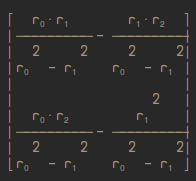
\includegraphics[width=0.45\textwidth]{./img/21-a.png}
\end{center}

\subsubsection{b}
\label{sec:orgf50f2a4}

\begin{verbatim}
p = [-a1; -a2];
R*r
\end{verbatim}

\begin{center}
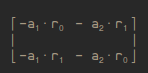
\includegraphics[width=0.45\textwidth]{./img/21-b.png}
\end{center}

Now solving for \(r_1\)

\begin{equation*}
\begin{array}{l}
r_1 + a_2 r_1 = -a_1 r_0 \\
r_1 = \frac{-a_1}{1+a_1}\sigma_y^2
\end{array}
\end{equation*}

Similarly for \(r_2\)

\begin{equation*}
\begin{array}{l}
r_2 = -a_1 r_1 - a_2 r_0 \\
r_2 = -a_1 (\frac{-a_1}{1+a_2}\sigma_y^2) a_2 \sigma_y^2 \\
r_2 = (\frac{a_1^2}{1+a_2} - a_2)\sigma_y^2
\end{array}
\end{equation*}

\subsubsection{c}
\label{sec:org4a508a3}

\begin{equation*}
\begin{array}{l}
\sigma_y^2 - a_1 \frac{a1}{1+a_2}\sigma_y^2 + a_2 (\frac{a_1^2}{1+a_2}-a_2)\sigma_y^2 \\
\sigma_y^2 - \frac{a1^2}{1+a_2}\sigma_y^2+ (\frac{a_1^2 a_2}{1+a_2}-a_2^2)\sigma_y^2 \\
\sigma_y^2 = \frac{\sigma_f^2}{1 - \frac{a_1^2}{1+a_2} + (\frac{a_1^2 a_2}{1+a_2}-a_2^2)}\\
\sigma_y^2 = (1+a_2)\frac{\sigma_f^2}{1+a_2 - a_1^2 + a_1^2 a_2-a_2^2(1+a_2)}\\
\sigma_y^2 = (1+a_2)\frac{\sigma_f^2}{(1-a_2)(a_2 + 1)^2 - a_1^2(1-a_2)} \\
\sigma_y^2 = \frac{1+a_2}{1-a}\frac{\sigma_f^2}{[(1+a_2)^2 - a_1^2]}
\end{array}
\end{equation*}

\subsubsection{d}
\label{sec:org53c9f9a}
Similarly to differential equations, we can write the solution of the difference equation in the form

$$
r_k = c_1 p_1^k + c_2 p_2^k
$$

Given the initial conditions \(r_0 = \sigma_y^2\) and \(r_1 = -\frac{a_1}{1+a_2}\sigma_y^2\). We can solve for \(c_1\) and \(c_2\).
Plugging \(r_0\) gives

\begin{equation*}
\sigma_y^2 = c_1 + c_2
\end{equation*}

Similarly for \(r_1\) we can start solving for \(c_1\) and \(c_2\)

\begin{equation*}
\begin{array}{l}
c_1 = \frac{a_1}{1+a_2}\sigma_y^2 - c_2 p_2 \\
\text{plug in to find} \\
c_2 = \frac{\sigma_y^2 p_1 - \frac{a_1}{1+a_1}\sigma_y^2}{p_1 - p_2} \\
\text{plug back into $c_1$ to get} \\
c_1 = \frac{a_1}{1+a_2}\sigma_y^2 - \frac{\sigma_y^2 p_1 - \frac{a_1}{1+a_1}\sigma_y^2}{p_1 - p_2} p_2 \\
\end{array}
\end{equation*}
\end{document}